\chapter{Marktformen und vollkommener Wettbewerb}

Wenn neue Unternehmen in eine Branche eintreten, steigt das Angebot, wodurch die (inverse) Angebotskurve flacher wird. Daraus folgt, dass der Gleichgewichtspreis sinkt und sich der Gewinn verringert. Wenn andererseits Unternehmen aus dem Markt austreten, wird die (inverse) Angebotskurve steiler. ~\bigskip

Gründe für Ein- oder Austritte können dabei kurzfristig sowohl ökonomische Gewinne als auch von ökonomische Verluste sein. Sobald jedoch eine Firma Verluste schreibt, so muss sie sich zuerst zwischen einem sogenannten Shutdown und einem tatsächlichen Marktaustritt entscheiden.
\begin{itemize}
	\item Die Entscheidung die Produktion lediglich temporär einzustellen (sog. \textbf{Shutdown}), d.h. $y = 0$, ist eine Entscheidung hinsichtlich der kurzen Frist. Eine solche Entscheidung macht Sinn, falls $p < AVC$.
	\item Falls der Preis langfristig allerdings unter den Durchschnittskosten bleibt, ist es für eine Unternehmung zur Vermeidung permanenter Verlust optimal, aus dem Markt auszutreten (sog. \textbf{Marktaustritt}). Das heißt, die Bedingung dazu ist $p < AC$.
\end{itemize}

\subsubsection*{Langfristiges Marktgleichgewicht}

Wie angesprochen kommt es bei ökonomischen Gewinnen zu Markteintritte und bei Verlusten zu Marktaustritten. Langfristig wird damit der ökonomische Gewinn gleich null sein und  jede Unternehmung produziert die \enquote{efficient scale}, i.e. $y = \arg \min AC(y)$; die langfristige Angebotskurve ist damit horizontal, Anpassungen in der langfristigen Gleichgewichtsmenge vollziehen sich durch Marktein- und austritte!

\begin{figure*}[!htbp] \centering
	\caption*{Zwei Technologien: A und B. Welche herrscht langfristig vor?}
	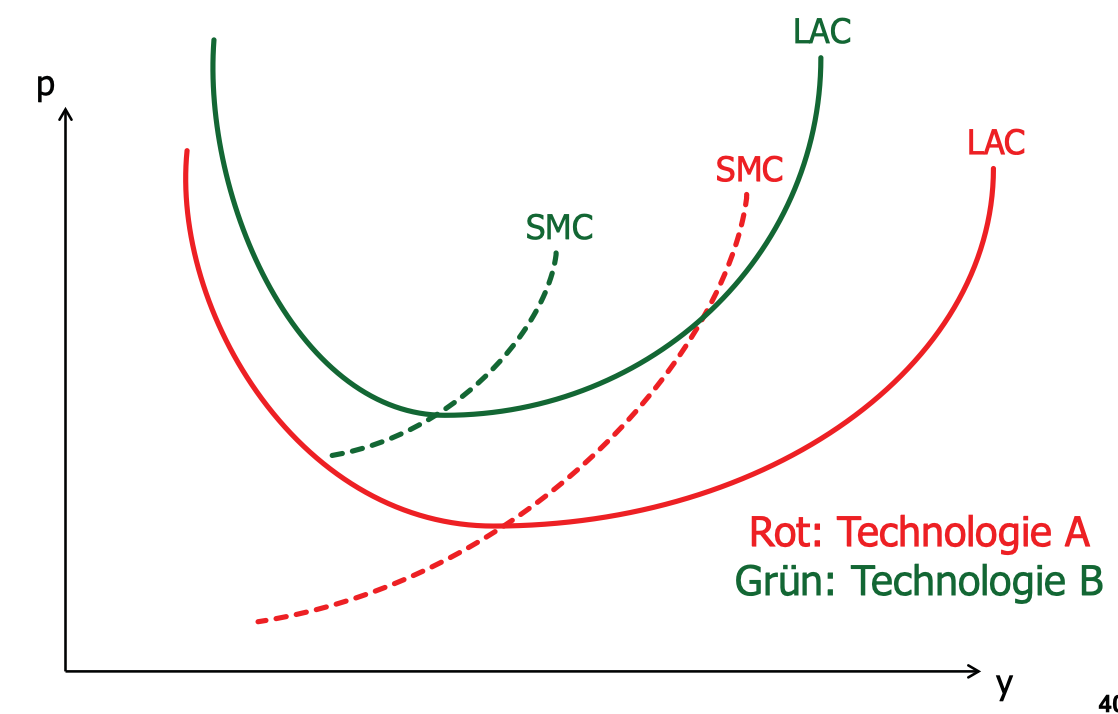
\includegraphics[scale=0.2425]{img/vwlm}
\end{figure*}

Betrachtet man allerdings einen Markt mit einer diskreten Anzahl an Unternehmungen, so werden offensichtlich nur so lange Firmen eintreten, bis die aus einem neuen Markteintritt resultierende Preissenkung in einem Verlust resultieren würde. Somit ist bei einer diskreten Marktgröße langfristig die Zahl der in einem Markt aktiven Unternehmungen durch $n^*$ gegeben, wobei bei $n^*$ aktiven Unternehmungen nichtnegative Gewinne vorliegen und bei $n^{*+1}$ Verluste entstehen. Die Produktionsmenge jeder Unternehmung ist dabei im diskreten langfristigen Marktgleichgewicht näherungsweise analog zu oben durch ihre effiziente Betriebsgröße $y^eff$ gegeben, bei der die Durchschnittskosten minimiert sind.

\subsubsection*{Vollkommener Wettbewerb}

Der vollkommener Wettbewerb ist ein theoretisches Modell, in dem ausreichend viele Anbieter, alle ohne Marktmacht und als Preisnehmer agierend, lediglich über ihre Angebotsmenge entscheiden. Jeder Anbieter maximiert somit bei festen Preis $p$ seinen Gewinn bezüglich $y$:
	$$ \max_y \Pi(y) = R(y) - C(y) = p \cdot y - C(y) $$
	
\begin{itemize}
	\item \textbf{Marginal Revenue}: Der Grenzerlös $MR(y)$ ist die erste Ableitung der Erlösfunktion $R(y)$.
	\item \textbf{Marginal Costs}: Die Grenzkosten $MC(y)$ die erste Ableitung der Kostenfunktion $C(y)$
	\item Im Gewinnmaximum gilt nach Bedingung erster Ordnung demnach: 
		$$ \text{Grenzerlös = Grenzkosten }~ (MR = MC) $$
\end{itemize}

Ein Unternehmen bietet also bei vollständiger Konkurrenz somit bei jedem Preis diejenige Menge an, bei der die Grenzkosten dem gegebenem Preis entsprechen. Dies ist die gewinnmaximierende Outputmenge.

\begin{kr}[Unternehmungen im vollkommenen Wettbewerb]
	Da bei vollkommendem Wettbewerb die Anbieter als Preisnehmer agieren, muss im Optimum gelten:
	$$ MC(y) = p(y) $$
	Auflösen dieser Gleichung nach $y$ ergibt die optimale Produktionsmenge.
\end{kr} 

